%%%%%%%%%%%%%%%%%%%%%%%%%%%%%%%%%%%%%%%%%
% Arsclassica Article
% LaTeX Template
% Version 1.1 (10/6/14)
%
% This template has been downloaded from:
% http://www.LaTeXTemplates.com
%
% Original author:
% Lorenzo Pantieri (http://www.lorenzopantieri.net) with extensive modifications by:
% Vel (vel@latextemplates.com)
%
% License:
% CC BY-NC-SA 3.0 (http://creativecommons.org/licenses/by-nc-sa/3.0/)
%
%%%%%%%%%%%%%%%%%%%%%%%%%%%%%%%%%%%%%%%%%

%----------------------------------------------------------------------------------------
%	PACKAGES AND OTHER DOCUMENT CONFIGURATIONS
%----------------------------------------------------------------------------------------

\documentclass[
10pt, % Main document font size
a4paper, % Paper type, use 'letterpaper' for US Letter paper
oneside, % One page layout (no page indentation)
%twoside, % Two page layout (page indentation for binding and different headers)
headinclude,footinclude, % Extra spacing for the header and footer
BCOR5mm, % Binding correction
]{scrartcl}

%%%%%%%%%%%%%%%%%%%%%%%%%%%%%%%%%%%%%%%%%
% Arsclassica Article
% Structure Specification File
%
% This file has been downloaded from:
% http://www.LaTeXTemplates.com
%
% Original author:
% Lorenzo Pantieri (http://www.lorenzopantieri.net) with extensive modifications by:
% Vel (vel@latextemplates.com)
%
% License:
% CC BY-NC-SA 3.0 (http://creativecommons.org/licenses/by-nc-sa/3.0/)
%
%%%%%%%%%%%%%%%%%%%%%%%%%%%%%%%%%%%%%%%%%

%----------------------------------------------------------------------------------------
%	REQUIRED PACKAGES
%----------------------------------------------------------------------------------------

\usepackage[
nochapters, % Turn off chapters since this is an article        
beramono, % Use the Bera Mono font for monospaced text (\texttt)
eulermath,% Use the Euler font for mathematics
pdfspacing, % Makes use of pdftex’ letter spacing capabilities via the microtype package
dottedtoc % Dotted lines leading to the page numbers in the table of contents
]{classicthesis} % The layout is based on the Classic Thesis style

\usepackage{arsclassica} % Modifies the Classic Thesis package

\usepackage[T1]{fontenc} % Use 8-bit encoding that has 256 glyphs

\usepackage[utf8]{inputenc} % Required for including letters with accents

\usepackage{graphicx} % Required for including images
\graphicspath{{Figures/}} % Set the default folder for images

\usepackage{enumitem} % Required for manipulating the whitespace between and within lists

\usepackage{lipsum} % Used for inserting dummy 'Lorem ipsum' text into the template

\usepackage{subfig} % Required for creating figures with multiple parts (subfigures)

\usepackage{amsmath,amssymb,amsthm} % For including math equations, theorems, symbols, etc

\usepackage{varioref} % More descriptive referencing

\usepackage{tabularx} % http://tex.stackexchange.com/questions/15282/tabular-title-above-and-caption-below
\usepackage{ragged2e}
\usepackage{booktabs}
\usepackage{caption}

\usepackage{url} % http://stackoverflow.com/questions/2640111/url-latex-linebreak-problem

%----------------------------------------------------------------------------------------
%	THEOREM STYLES
%---------------------------------------------------------------------------------------

\theoremstyle{definition} % Define theorem styles here based on the definition style (used for definitions and examples)
\newtheorem{definition}{Definition}

\theoremstyle{plain} % Define theorem styles here based on the plain style (used for theorems, lemmas, propositions)
\newtheorem{theorem}{Theorem}

\theoremstyle{remark} % Define theorem styles here based on the remark style (used for remarks and notes)

%----------------------------------------------------------------------------------------
%	HYPERLINKS
%---------------------------------------------------------------------------------------

\hypersetup{
%draft, % Uncomment to remove all links (useful for printing in black and white)
colorlinks=true, breaklinks=true, bookmarks=true,bookmarksnumbered,
urlcolor=webbrown, linkcolor=RoyalBlue, citecolor=webgreen, % Link colors
pdftitle={}, % PDF title
pdfauthor={\textcopyright}, % PDF Author
pdfsubject={}, % PDF Subject
pdfkeywords={}, % PDF Keywords
pdfcreator={pdfLaTeX}, % PDF Creator
pdfproducer={LaTeX with hyperref and ClassicThesis} % PDF producer
} % Include the structure.tex file which specified the document structure and layout

\hyphenation{Fortran hy-phen-ation} % Specify custom hyphenation points in words with dashes where you would like hyphenation to occur, or alternatively, don't put any dashes in a word to stop hyphenation altogether

%----------------------------------------------------------------------------------------
%	TITLE AND AUTHOR(S)
%----------------------------------------------------------------------------------------

\title{\normalfont\spacedallcaps{Whitehouse.gov usability report}} % The article title

\author{\spacedlowsmallcaps{Enrico Rotundo*, 1008052}} % The article author(s) - author affiliations need to be specified in the AUTHOR AFFILIATIONS block

\date{August, 2014} % An optional date to appear under the author(s)

%----------------------------------------------------------------------------------------

\begin{document}

%----------------------------------------------------------------------------------------
%	HEADERS
%----------------------------------------------------------------------------------------

\renewcommand{\sectionmark}[1]{\markright{\spacedlowsmallcaps{#1}}} % The header for all pages (oneside) or for even pages (twoside)
%\renewcommand{\subsectionmark}[1]{\markright{\thesubsection~#1}} % Uncomment when using the twoside option - this modifies the header on odd pages
\lehead{\mbox{\llap{\small\thepage\kern1em\color{halfgray} \vline}\color{halfgray}\hspace{0.5em}\rightmark\hfil}} % The header style

\pagestyle{scrheadings} % Enable the headers specified in this block

\sloppy % solve the problem with overfull boxes (e.g. \href over the hbox)

%----------------------------
% CUSTOM COMMAND
%----------------------------

\newcommand{\thesite}{\href{http://www.whitehouse.gov/}{whitehouse.gov}}

\newcolumntype{C}[1]{>{\Centering}m{#1}} % http://tex.stackexchange.com/questions/15282/tabular-title-above-and-caption-below
\renewcommand\tabularxcolumn[1]{C{#1}}

%----------------------------------------------------------------------------------------
%	TABLE OF CONTENTS & LISTS OF FIGURES AND TABLES
%----------------------------------------------------------------------------------------

\maketitle % Print the title/author/date block

\setcounter{tocdepth}{2} % Set the depth of the table of contents to show sections and subsections only

\tableofcontents % Print the table of contents

\listoffigures % Print the list of figures

% \listoftables % Print the list of tables

%----------------------------------------------------------------------------------------
%	ABSTRACT
%----------------------------------------------------------------------------------------

%\section*{Abstract} % This section will not appear in the table of contents due to the star (\section*)

%\lipsum[1] % Dummy text

%----------------------------------------------------------------------------------------
%	AUTHOR AFFILIATIONS
%----------------------------------------------------------------------------------------

{\let\thefootnote\relax\footnotetext{* \textit{Computer Science BSc student, AY 2013-2014, Department of Mathematics, University of Padua, Italy}}}

%----------------------------------------------------------------------------------------

\newpage % Start the article content on the second page, remove this if you have a longer abstract that goes onto the second page

%----------------------------------------------------------------------------------------
%	INTRODUCTION
%----------------------------------------------------------------------------------------

\section{Introduction}
	This documents is a usability report of the website \thesite{}, following referred as ``the site'' or ``the website''. The website analyzed represent the US government, it's focused on the person of the President and delivers high grained information about him and Administration's activities.  
 
%----------------------------------------------------------------------------------------
%	NAME AND DOMAIN
%----------------------------------------------------------------------------------------

\section{Name and domain}

The website's name is the same of the institutions that represents, its meaning is unambiguous all around the world, so it's enough well-known to be clear and immediate. The domain is \emph{.gov}, clearly represents an official government website, so its choice is appropriate. Others domains, like \emph{.com}/\emph{.org}/\emph{.it}, don't redirect to \thesite{} and seems to be not related to the government. Since the website is a sensible target, i would expect that at least the \emph{.com} redirects to the main one, simply to avoid possible attacks like website cloning.

%----------------------------------------------------------------------------------------
%	HOMEPAGE
%----------------------------------------------------------------------------------------

\section{Homepage}
\label{homepage}

\begin{figure}[p]
\centering 
\centerline{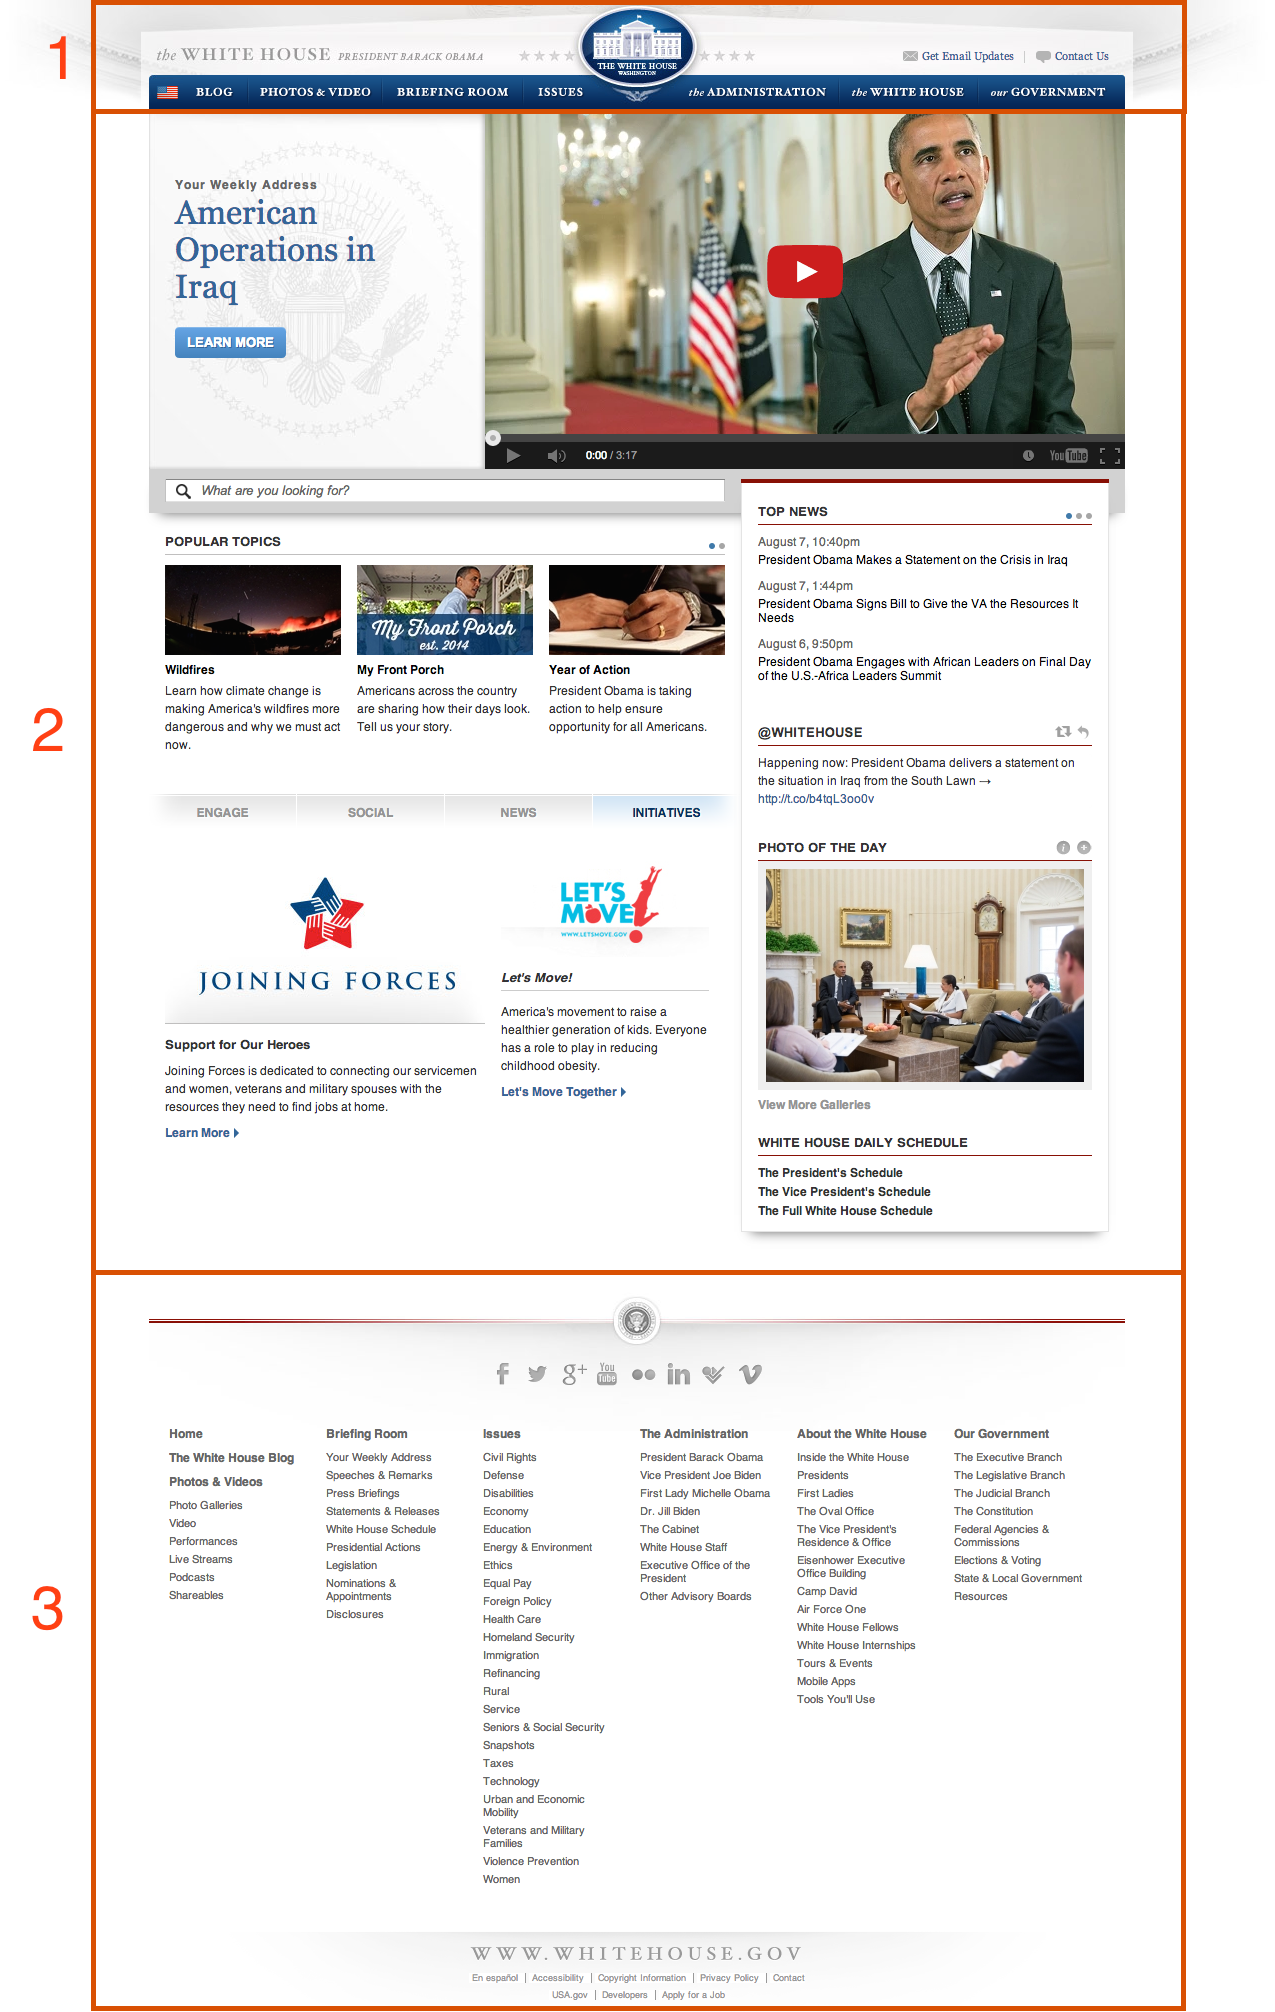
\includegraphics[width=1.4\columnwidth]{homepage-entire-sections}}
\caption[Homepage]{Homepage of \thesite{}. 1 header, 2 body, 3 footer.}
\label{fig:homepage} 
\end{figure}

The first view of the homepage (Figure \ref{fig:homepage}) has a scanning time enough low to shows the 6w's\footnote{included ``How'', \url{http://en.wikipedia.org/wiki/Five_Ws}} by the limit time\footnote{30 seconds}.

\begin{itemize}%[noitemsep]
	\item \textbf{Where:} where are we? \\ The subtitle isn't so descriptive but the words \emph{whitehouse} and \emph{President Barack Obama} together clarify where we are. The breadcrumb lack doesn't tell us where we are inside the website, this create user's disorientation;

	\item \textbf{Who:} who represents the site? \\ In the top-left, a subtitle explaining that the whitehouse's representative is the President Barack Obama; that's an image and not plain text, this doesn't respect the common web rules, invalidating text advantages. \\
	The whitehouse logo is in the top-center and includes a graphical text mentioning, another time, the white house. It correctly links to the homepage but a negative note is about the size: text is too small and image size doesn't respect the \emph{target size rule}\footnote{the more important a button is, the bigger it should be.}; I believe that the whitehouse logo is enough important (also as homepage link) to deserve a bigger size;

	\item \textbf{Why:} why should i remain in this website? \\ This isn't a commercial website so we are interested in public domain infos about the white house. There're daily updates about relevant political facts, usually located in the central slide-show and in below sections;

	\newpage
	\item \textbf{What:} what offers the site? \\ This site offers information for citizens, from the President's activity to issues like economy, taxes, defense and political reports;

	\item \textbf{When:} this is about temporal references contained into the site. \\ The ``top news'' section contains frequently updated news and the central slide-show offers last facts updates, often supplied with media (e.g., picture, video); 

	\item \textbf{How:} how we can move across the website? \\ The menu is top centered and has a good centered and wide sub-menus. There's also a search bar at the bottom of the central slide-show.

\end{itemize}

Homepage can be divided in the following sections as in Figure \ref{fig:homepage}:
	
	\begin{enumerate}
		
		\item \textbf{Header:} logo and website's subtitle are well located in the ``hot'' top-left area, they correctly links to the homepage. Contacts buttons (i.e. get email updates, contact us) are properly colored as link and the link area includes the icons. \\
		US flags located in the left menu confuse users, indeed it redirects to the homepage while flags are often (wrongly\footnote{\href{http://flagsarenotlanguages.com}{http://flagsarenotlanguages.com}}) associated with language selector. \\
		Submenus're wide and don't unexpectedly disappears when user interacts with them, a bit bothersome are those advertisement-like columns, they've imgs so distract users in sub-menu scanning;
		
		\item \textbf{Body:} top body has wide area with some text and media, the button is correctly non-graphical and video length variance is very high, depends on day, but generally there're videos longer then 3 minutes. This is allowed for a \emph{.gov} site but it has to be said that propose a 32mins\footnote{in date 2014-08-08} video in homepage couldn't be a wise choice. Search toolbar is discussed in \ref{searchtools}. \\
		Popular topics section lacks in title link color and the buttons to navigate across topics are too small and require precise mouse pointing, not very comfortable for users. It's correct that imgs are links and slightly brighten up on the mouse over. Below there's a tab selector, tabs navigation is clear, images are all clickable but sometimes too small. \\
		Top news section hasn't any colored links and lacks on the same issue, mentioned above, on news navigation. Curious are the icons 
\includegraphics[scale=0.6]{social-rows} in the social area, for a non-\emph{twitter} users is difficult to understand their meaning also because they lead to the same splash screen (discussed in \ref{splashpage}). Another note goes to the photo of the day section icons 
\includegraphics[scale=0.6]{day-photo-home}, indeed while the plus button enlarge the photo, the info icon isn't a button, it overlays textual infos over the picture but isn't clickable, so user is confused and ends to click on it multiple times, browser selects it and result is unaesthetic;
		
		\item \textbf{Footer:} on the top there're social icons dominated by the seal of the President icon; while socials are clickable the latter isn't so we have different behavior of near icons, this confuse users.
		Footer height is over-sized due the \emph{issue} column that's higher than the average. The bottom image \emph{www.whitehouse.gov} is just an image and doesn't links to the cited website, furthermore the bottom word's font is too small, 9px, against a lower-bound limit allowed of 10px. 
		
	\end{enumerate}

%----------------------------------------------------------------------------------------
%	INTERNAL PAGES
%----------------------------------------------------------------------------------------

\section{Internal pages}
Most of internal pages are structured in base of the sub-level: 2\textsuperscript{nd} and 3\textsuperscript{rd} levels have their own layout.
All sub-levels, except homepage, have a \emph{location breadcrumb} located at the bottom of the menu: it shows your position relative to the homepage. Inline with the breadcrumb there's the search bar, the textbox allows 25 chars before to run into the \emph{guillotine effect}\footnote{when textbox are too small so users are forced to use scrollbars to show up the content.}; furthermore the search tool shows a clear \emph{search} button instead to require a click on the hand lens. 
Every page seems to be reachable from the homepage in most 3 clicks, that's why the menu is complete and well done. 
Internal pages are reachable from different pages than the home (\emph{deep linking}) so they have to propose again the compulsory informative axis: \emph{who}/\emph{what}/\emph{where}, the website correctly respects this requirement.
Below there're the analysis of three subpages.

	\subsection{/briefing-room}
	\label{primapaginainterna}
	

	\begin{figure}[h!]
	\centering 
	\centerline{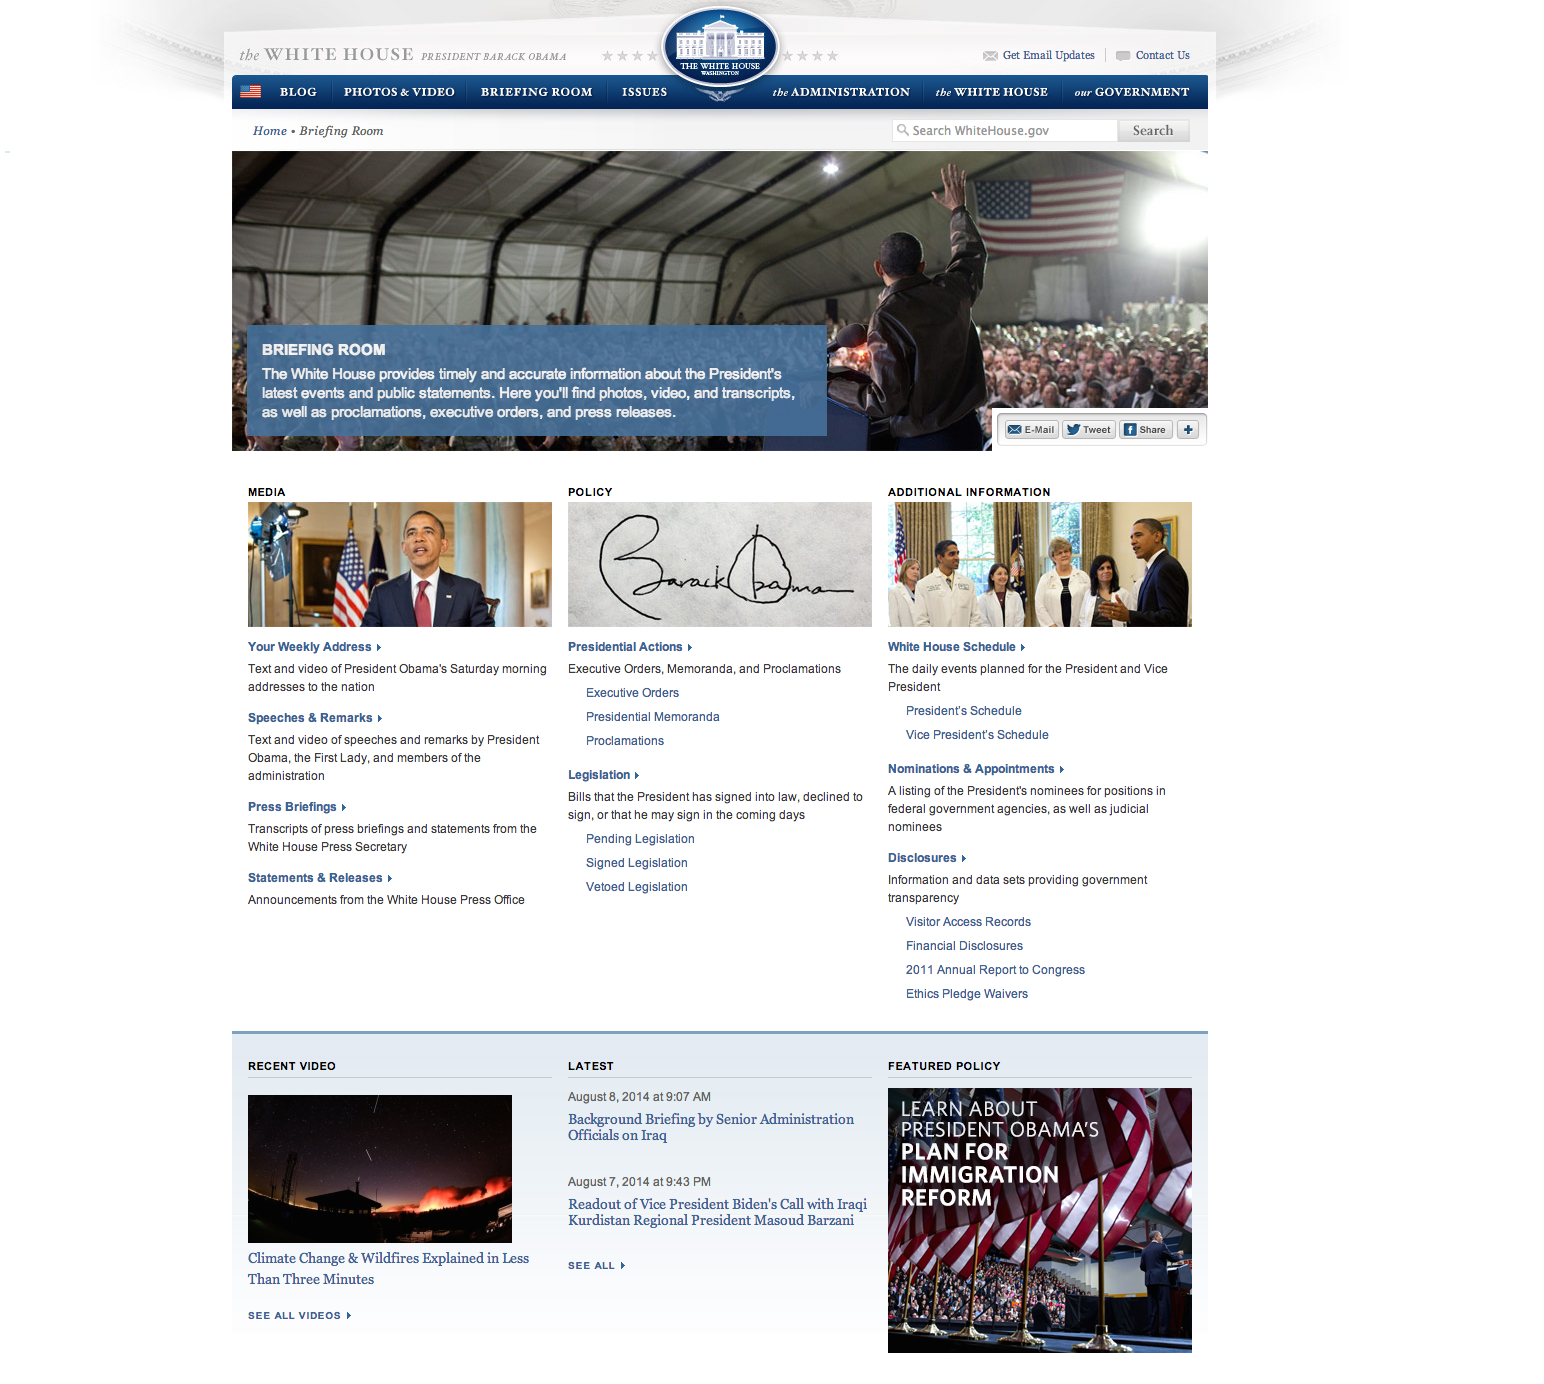
\includegraphics[width=2\columnwidth]{1-internal-page-entire}}
	\caption[First internal page: /briefing-room]{First internal page: \emph{/briefing-room}.}
	\label{fig:primapaginainterna} 
	\end{figure}

	The briefing room page (Figure \ref{fig:primapaginainterna}) (\href{http://www.whitehouse.gov/briefing-room}{whitehouse.gov/briefing-room}) provides information about the President's activity, latest events and public statements. The page has a top-central image that immediately recalls a President's public speech. A text subtitle explain what kind of page is, that's good because accomplishes the \emph{where} compulsory axis meanwhile permits the \emph{common text operations}\footnote{select, copy, paste.}, furthermore a set of social icons are well visible to share contents. \\
	The page content is divided in three columns, that's make user scanning effort more demanding but maybe authors wanted to put on the same footing those contents (media, policy, additional infos). Images are a bit short in height (304x125px) but sufficiently big to show their contents, they aren't links so click over doesn't produce any effects, this is undesirable since imgs appeals clicks. \\
	Text content is well separated in short and titled blocks, that's very good, furthermore every title is a colored link. The overall height and structure is enough compact to ensure a rapid scan. \\
	A three columns bottom-content frame is located at the bottom page. Columns are \emph{recent video}, \emph{latest} and \emph{featured policy}. The first one shows a clickable thumbnail and a subtitle, the image is 274x153px, clearly too small to be exhaustive. The second one presents a list of news with a precise temporal reference. The last one has always a 311x272px clickable image, big enough.

	\newpage
	\subsection{/briefing-room/legislation}
	\label{secondapaginainterna}

	\begin{figure}[h!]
	\centering 
	\centerline{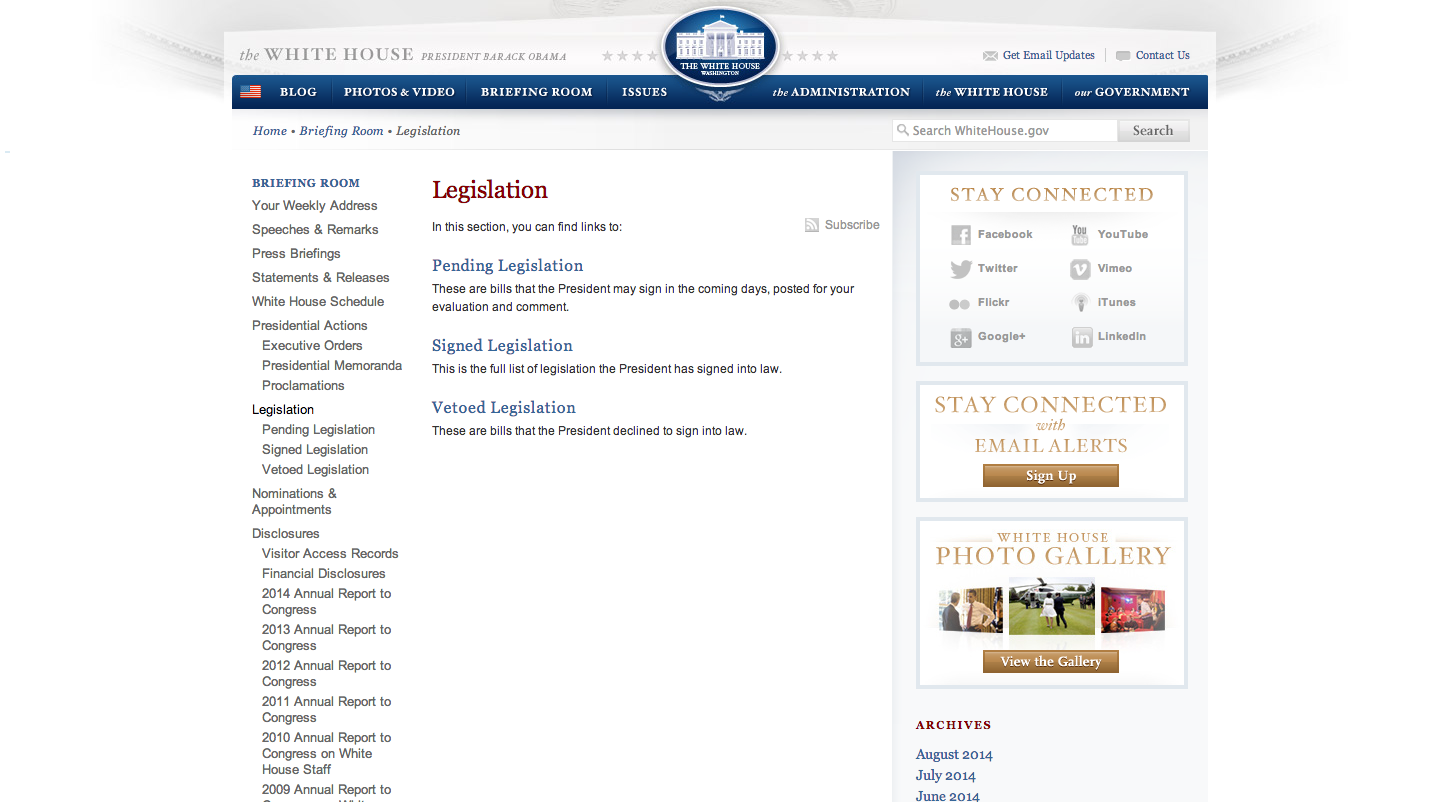
\includegraphics[width=2\columnwidth]{2-internal-page-visible}}
	\caption[Second internal page: /briefing-room/legislation]{Second internal page: \emph{/briefing-room/legislation}.}
	\label{fig:secondapaginainterna} 
	\end{figure}

	
	The legislation page (Figure \ref{fig:secondapaginainterna}) (\href{http://www.whitehouse.gov/briefing-room/legislation}{whitehouse.gov/briefing-room/legislation}) is a 3\textsuperscript{rd} sublevel page. This page shows links to three kind of legislation (pending, signed, voted). There's no top images. Layout has three columns structure, this isn't a good practice because users can't easily scan it. On the left side there's a menu (\textbf{1}) for the whole \emph{briefing room} section showing every section sublevels. Its height is suited for nowadays content but the voice \emph{Disclosures} contains annuals reports so it's expected to grow every year; this could produce user dissatisfaction so it's clear that there's an early design lack. Another bad note is colored links absence. \\
	The central column shows a good design, with a clear main title, short subtitle and a compact list of minor titles with short description. \\
	The right side column is a bit problematic. First, there are three frame containing graphical text. Second, the \emph{Archives} section (\textbf{2}) is an example of \emph{lorem ipsum damnation}: probably in design time it was filled with a short example content (e.g., lorem ipsum), then with the passing of the time it grew up a lot; this is an early design defect that'll cause trouble to users, what about within ten years?
	

	\subsection{/issues/technology}
	\label{terzapaginainterna} 

	
	The technology page (Figure \ref{fig:terzapaginainterna}) (\href{http://www.whitehouse.gov/issues/technology}{whitehouse.gov/issues/technology}) is a 3\textsuperscript{rd} sublevel page. This page is an article about President's view of technology and explains the whitehouse's guideline principles. There's no top images; three column layout. In left side there's a menu showing only the first level of \emph{issues's} section. This choice is different between the previous page (\ref{secondapaginainterna}), maybe because it'd be so high. Another time, links aren't colored, this could confuse users. \\

	\begin{figure}[h!]
	\centering 
	\centerline{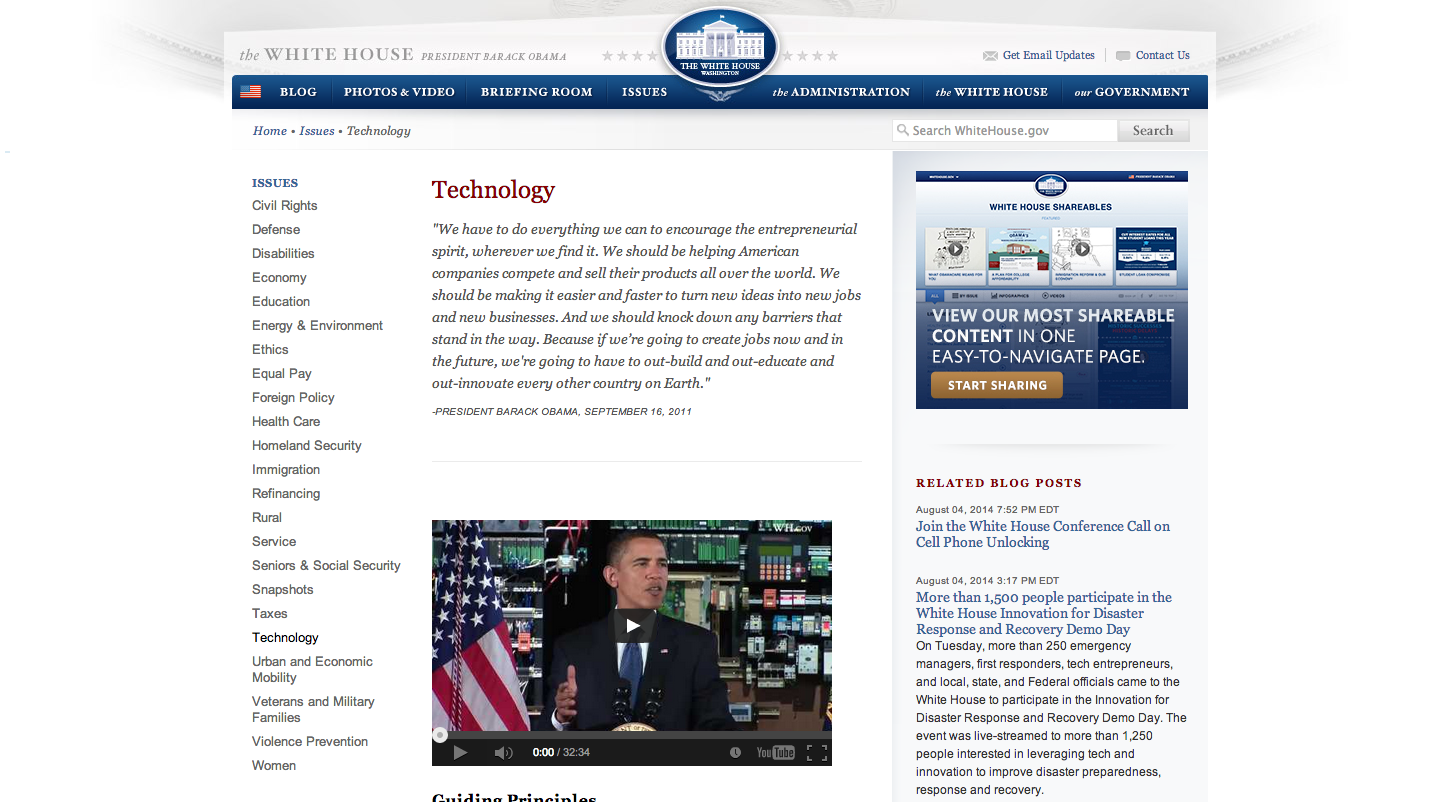
\includegraphics[width=2\columnwidth]{3-internal-page-visible}}
	\caption[Third internal page: /issues/technology]{Third internal page: \emph{/issues/technology}.}
	\label{fig:terzapaginainterna} 
	\end{figure}

	The central column has a clear title but a too long subtitle; a video with no clear title come first text, it's length is very long (32 mins). Text content isn't well organized: long text blocks\footnote{total 3790 words, reading takes 15-25 min.} with small titles, it could be divided in more than one pages. Text block is so long so at the bottom page there's a link to jump to the top. Social sharing icons are located at the end of the content, it'll take some time to spot it, this's undesirable in the web 2.0 era where a fast content sharing is required. \\
	The right column shows a 272x238px img with a fake button inside that isn't so intuitive for users. About the image size is ok. Then there're some related blog posts well presented, with colored links title and temporal reference. Next, related videos section take the place, thumbnails are too small (274x153px) and, in conflict with the previous section, titles are placed below the video thumbnail.
	
	\begin{figure}[h!]
	\centering 
	\centerline{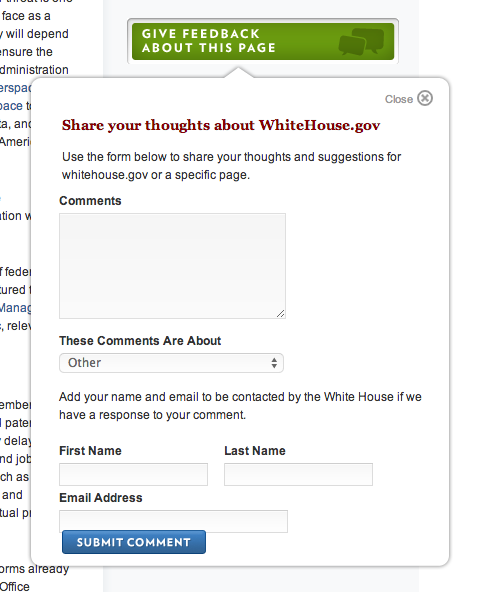
\includegraphics[width=0.8\columnwidth]{3-internal-page-detail}}
	\caption[feedback-form]{feedback-form included in every 3\textsuperscript{rd} sublevel page.}
	\label{fig:terzapaginainternadettaglio} 
	\end{figure}

	A black mark goes to the feedback-form shown in Figure \ref{fig:terzapaginainternadettaglio}, although it has a clear usage and has a limited number of inputs, its design is a bit strange. The comments text-box cannot be enlarged even though there's some empty space on the right. The way of escape is clear, a \emph{close} text button in upper right corner, however users would expect to close this form by clicking outside it, but it doesn't works in that way. Furthermore, the feedback-form behavior is confusing: clicking the green \emph{give feedback about this page} button (another time, an img button with non-text inside) to show up the form, users have to wait a too long delay before the form shows up; this happens also when user wants to close the form by clicking the green button.

%----------------------------------------------------------------------------------------
%	GENERALS OBSERVATIONS
%----------------------------------------------------------------------------------------

\newpage
\section{General observations}

	\subsection{Images}
	The majority of images can be clicked but there are pages (e.g., \ref{primapaginainterna}) with no clickable images. This disorientate users, especially in this site where the most part if imgs are clickable, indeed user have to understand by the context if he can click over an image.
	Image sizing is generally small, around or below the 210x230px limit, but important images are always big enough to be understood.

	\subsection{Texts}
	Text is visible, clear, big enough, always well contrasted relative to the background. There aren't no sizing buttons and there're too many fonts, sometimes more than 4 (e.g., \ref{terzapaginainterna}).
	There's an abuse of images containing texts and buttons, this cause user's dissatisfaction. 
	There're upper-case sentences, sometimes used as subtitle, but those number is not noteworthy. No keywords highlighted in bold.

	\subsection{Links}
	Links aren't always colored and visited links doesn't change color. This goes against web conventions and increase the user effort during navigation. 

	\subsection{Scroll}
	Page's height is well sized for the high level pages (e.g., 1\textsuperscript{st}, 2\textsuperscript{nd}) but going in deep reveals pages too high. Let's compare the homepage height with a 3\textsuperscript{rd} level page (\ref{terzapaginainterna}). \\
	Entire homepage is shown in Figure \ref{fig:entirehomepage}, the whole content fits in the first two screens, considering that the 3\textsuperscript{rd} screen is due to the \emph{issues} column, this is acceptable.
	A bad mark goes to the 3\textsuperscript{rd} level page (\ref{terzapaginainterna}) which is 9752px high: with a 1440x900px monitor, users needs to scroll 11 entire screens; unacceptable, it'd better to separate content in different tabs. 

	\begin{figure}[h]
	\centering 
	\centerline{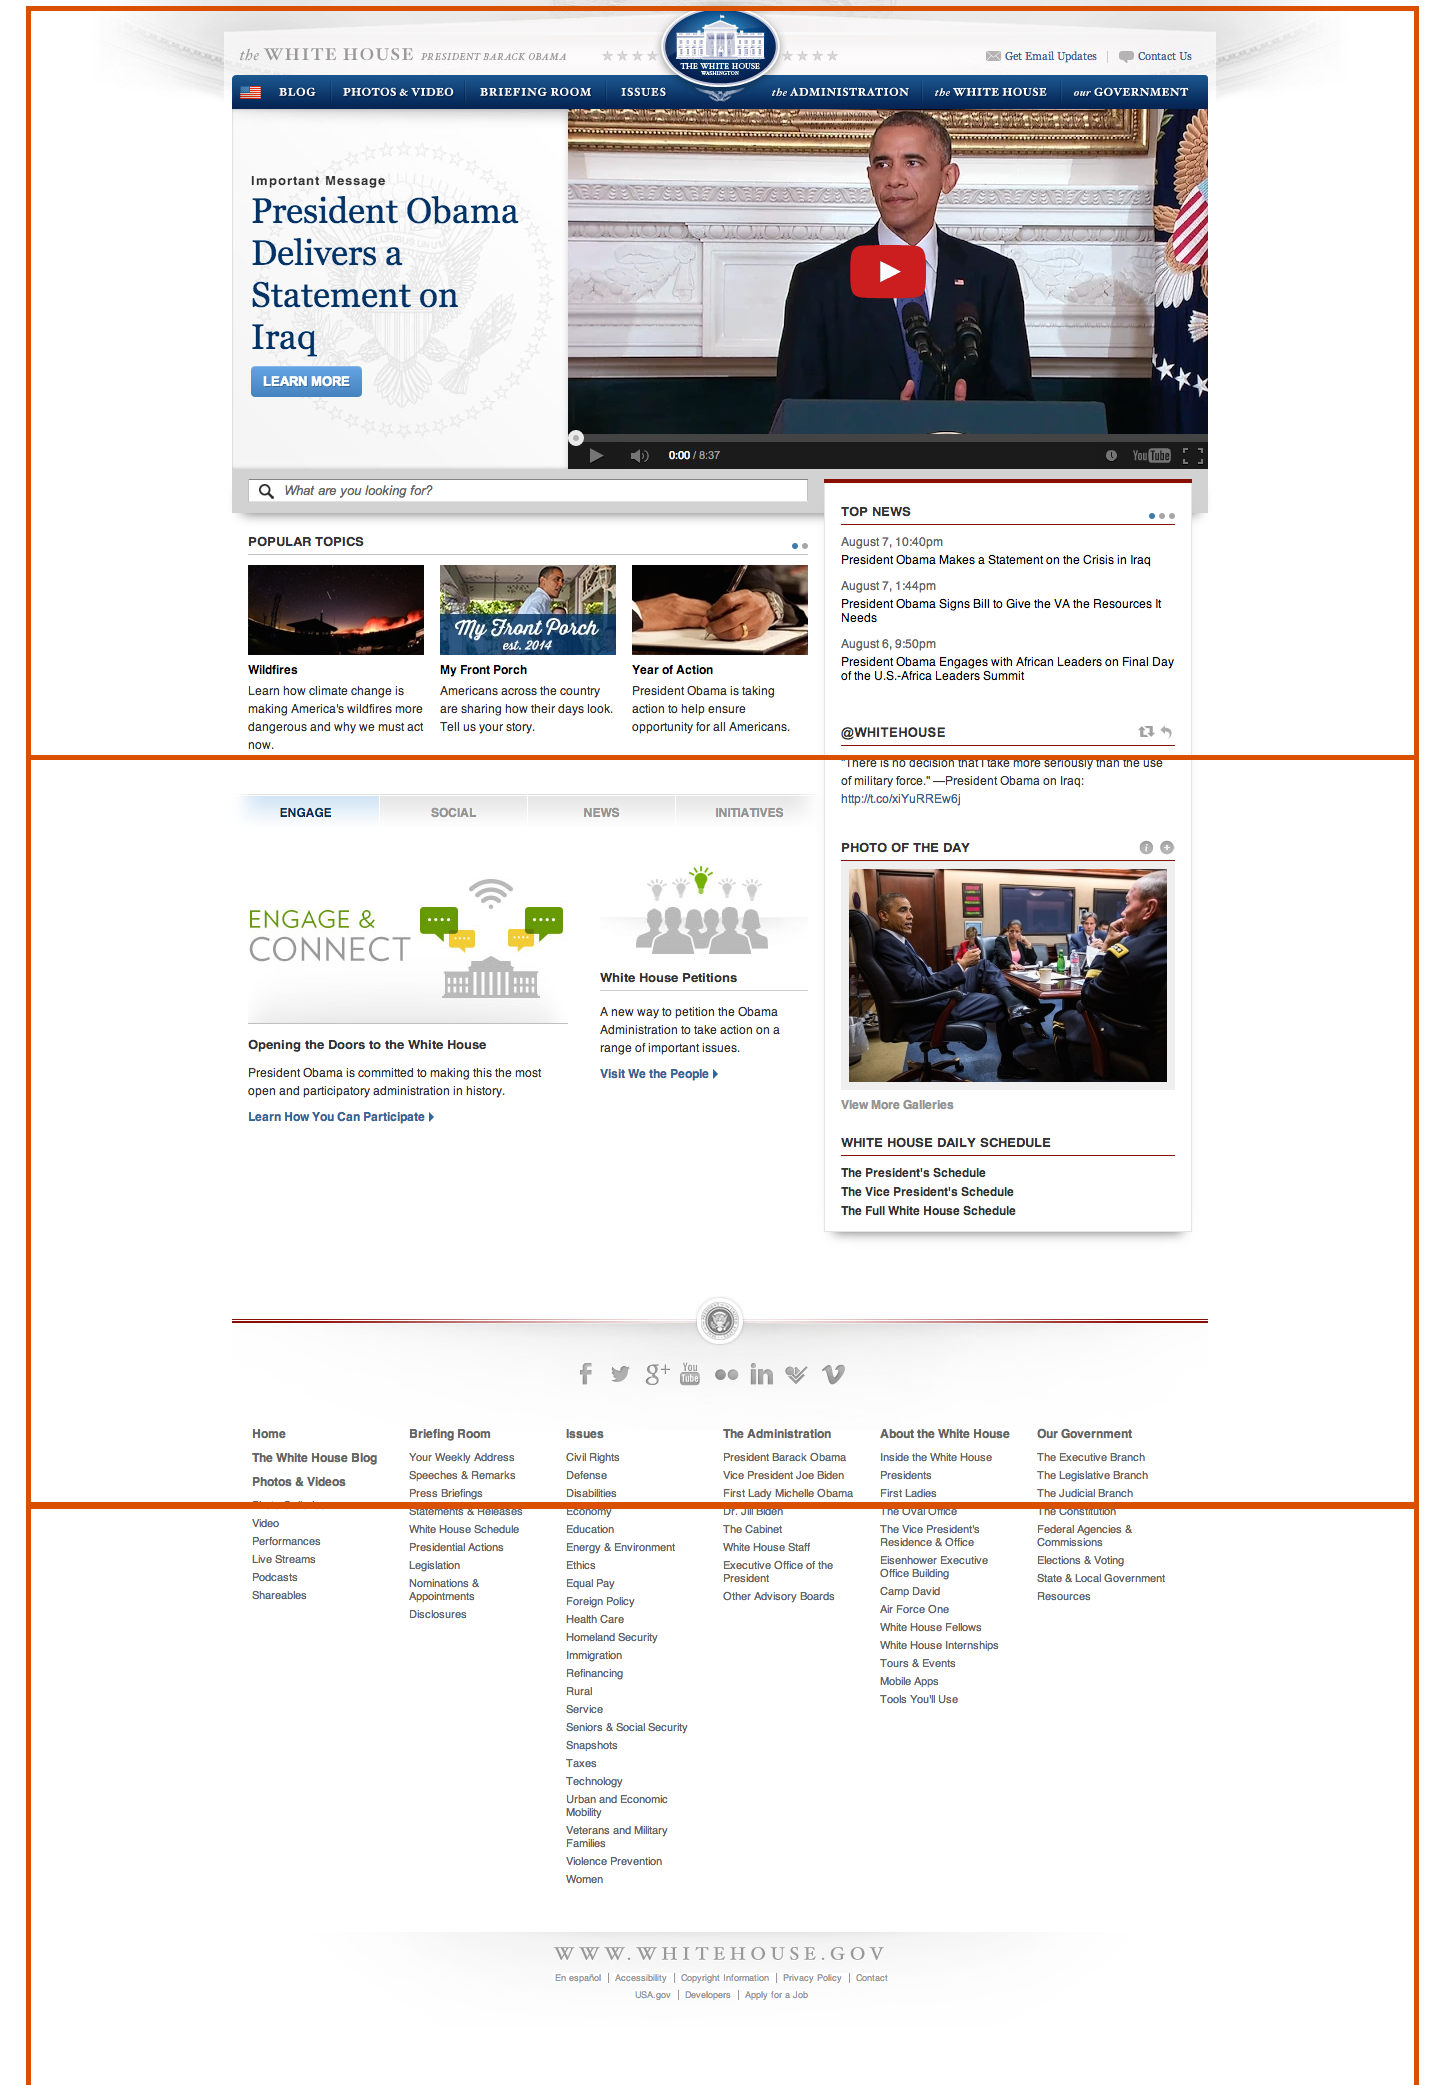
\includegraphics[width=0.9\columnwidth]{homepage-entire-screen}}
	\caption[Screen divided homepage]{Entire Homepage divided by 900px height screen.}
	\label{fig:entirehomepage} 
	\end{figure}

	\newpage
	\subsection{Search tools}
	\label{searchtools}
	Due to the website size, a search tool is present. The site uses Bing\footnote{\href{http://en.wikipedia.org/wiki/Bing}{http://en.wikipedia.org/wiki/Bing}} as search engine, but the research seems to be personalized for White House requirements. We can consider it as local search, indeed there's no redirects to the search engine page. The only reference to the external search engine is at the bottom page, an unclickable logo says: ``\emph{results by Bing}''. \\
	Search toolbar in pages is different from homepage (\ref{homepage}) and subpages (\ref{primapaginainterna}, \ref{secondapaginainterna}, \ref{terzapaginainterna}). The first one is located below the central wide image, the search button is an hand lens icon (bad); subpages has search bar above the central image, this time with the proper \emph{Search} button. Either search leads to the same results page (Figure \ref{fig:search-simple}). In case of an unsuccessful search, website correctly warns users with a message (Figure \ref{fig:search-no-results}).

	\begin{figure}[h]
	\centering 
	\centerline{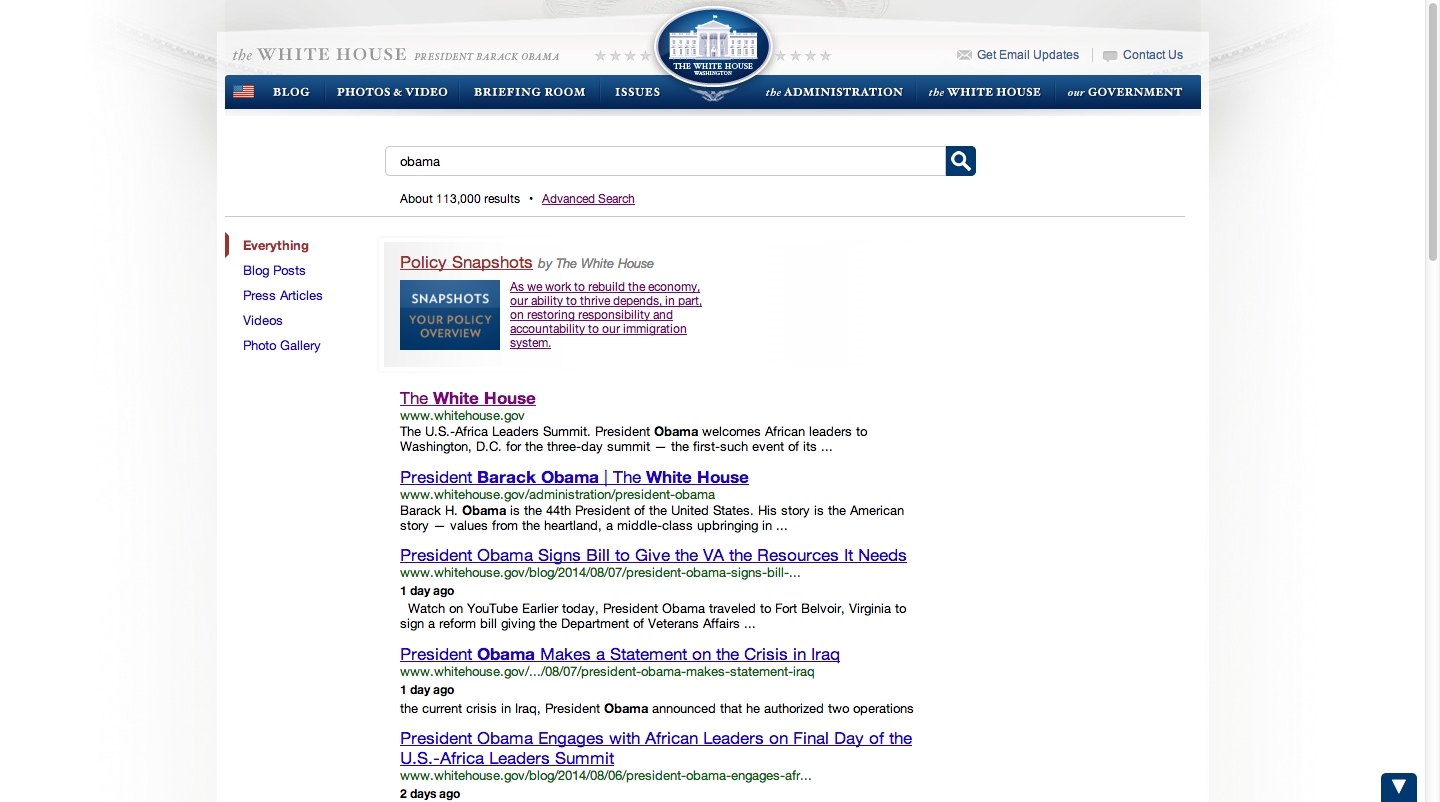
\includegraphics[width=2\columnwidth]{search-simple}}
	\caption[Simple search results page]{Simple search results page.}
	\label{fig:search-simple} 
	\end{figure}

	\begin{figure}[h]
	\centering 
	\centerline{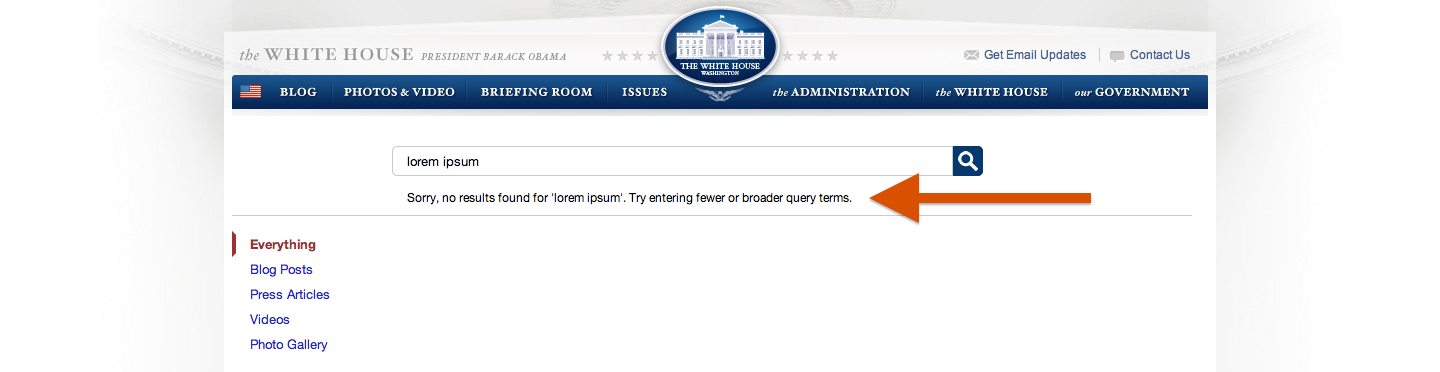
\includegraphics[width=2\columnwidth]{search-no-results}}
	\caption[No results search results page]{No results search results page.}
	\label{fig:search-no-results} 
	\end{figure}

	Advanced search (Figure \ref{fig:search-advanced}) is reachable from a simple search result page (Figure \ref{fig:search-simple}), this makes advanced search optional and is a positive mark. Notable is the restricted number of selection filters, but an unexplained \emph{safe search} make hard to understand what exactly means. Search button instead of the hand lens icon is considered good.


	\begin{figure}[h]
	\centering 
	\centerline{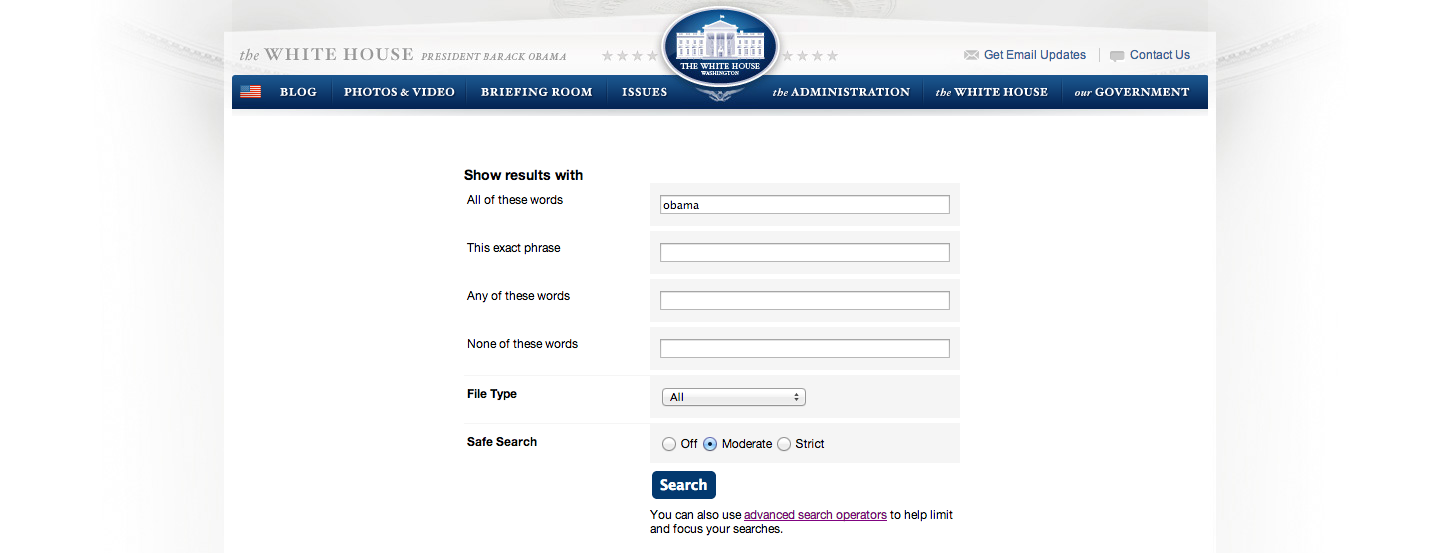
\includegraphics[width=1.8\columnwidth]{search-advanced}}
	\caption[Advanced search page]{Advanced search page}
	\label{fig:search-advanced} 
	\end{figure}

	\newpage
	\subsection{Back button}
	Back button works as expected in every page, never opens previous pages in a detached window.

	\newpage
	\subsection{Splash page}
	\label{splashpage}
	At the first visit there aren't any splash screens or registration form, nevertheless a splash screen (Figure \ref{fig:splash-screen}) appears when user click on an external link, in this case a message warns user that is leaving the \thesite{} web server. This message is very annoying and it goes against the web conventions.

	\begin{figure}[h]
	\centering 
	\centerline{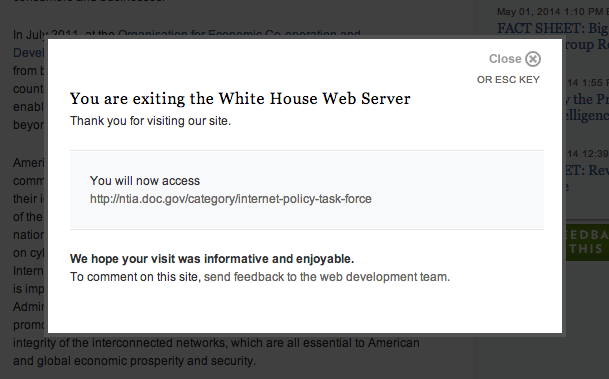
\includegraphics[width=1\columnwidth]{splash-screen}}
	\caption[Splash screen]{Splash screen appears when leaving \thesite{}.}
	\label{fig:splash-screen} 
	\end{figure}

	\subsection{Ads}
	This isn't a commercial website, nevertheless the site has some ads to specific themes (e.g., join military forces, taxes calculator). Ads are correctly located in the right column and gracefully integrates the site look. Although there aren't awful effects like blinking, rotating or on the move texts, it has to be said that sometimes whole ads images are clickable, sometimes only a portion. This clearly confuse users that usually try to click over images.

	\subsection{404}
	Inserting an invalid url the website correctly shows an error message (Figure \ref{fig:not-found-page}). This scenario happens when a user follows a broken link, the site properly invites to return to the homepage by a link. 

	\begin{figure}[t]
	\centering 
	\centerline{
\includegraphics[width=1.5\columnwidth]{404}}
	\caption[Not found page]{Error 404: not found page message.}
	\label{fig:not-found-page} 
	\end{figure}

%----------------------------------------------------------------------------------------
%	SUMMARY
%----------------------------------------------------------------------------------------

\clearpage
\section{Summary}
	\begin{centering}
	{ \huge \bfseries grade: 7.5/10 \\[0.3cm] }
	\end{centering}
	Considering the huge size of the site, the few defects identified and the complexity and variety of content delivered by \thesite{}, i consider it as a well designed website. Except the excessive height of some pages, defects detected are not so heavy to spoil navigation.


%----------------------------------------------------------------------------------------
%	LIST OF FIGURES
%----------------------------------------------------------------------------------------

\section{List of figures with file references}
Table below associate url's with image files used in this document:


	% \begin{table}[h]
	% 	\caption{List of figures with file references} % title of Table
	% 	\centering % used for centering table
	% 	\begin{tabular}{l l l} % centered columns (3 columns)
	% 		\hline\hline %inserts double horizontal lines
	% 		Figure & File name & URL \\ [0.5ex] % inserts table 
	% 		%heading
	% 		\hline % inserts single horizontal line
	% 			Homepage & homepage-entire-sections.png & \href{http://www.whitehouse.gov/}{link} \\ [1ex]
	% 			First internal page: /briefing-room & 1-internal-page-entire.png & \href{http://www.whitehouse.gov/briefing-room}{link}\\ [1ex]
	% 			Second internal page: /briefing-room/legislation & 2-internal-page-visible.png & \href{http://www.whitehouse.gov/briefing-room/legislation}{link} \\ [1ex]
	% 			Third internal page: /issues/technology & 3-internal-page-visible.png & \href{http://www.whitehouse.gov/issues/technology}{link} \\ [1ex]
	% 			feedback-form & 3-internal-page-detail.png & \href{http://www.whitehouse.gov/issues/technology}{link} \\ [1ex]
	% 			Screen divided homepage & homepage-entire-screen.png & \href{http://www.whitehouse.gov/}{link} \\ [1ex]
	% 			Simple search results page & search-simple.png & \href{http://stackoverflow.com/questions/2640111/url-latex-linebreak-problem}{link} \\ [1ex]
	% 			No results search results page & search-no-results.png & \href{http://search.whitehouse.gov/search?utf8=%E2%9C%93&query=lorem+ipsum&m=&affiliate=wh&commit=Search}{link} \\ [1ex]
	% 			Advanced search page & search-advanced.png & \href{http://search.whitehouse.gov/search/advanced?affiliate=wh&enable_highlighting=true&per_page=20&query=obama}{link} \\ [1ex]
	% 			Splash screen & splash-screen.png & \href{http://www.whitehouse.gov/issues/technology}{link} \\ [1ex]
	% 			Not found page & 404.png & \href{http://www.whitehouse.gov/admin}{link} \\ [1ex]
	% 			 % &  &  \\ [1ex]
	% 			 % &  &  \\ [1ex]
	% 			 % &  &  \\ [1ex]
	% 			 % &  &  \\ [1ex]
	% 			 % &  &  \\ [1ex]
	% 			 % &  &  \\ [1ex]
	% 		\hline %inserts single line
	% 	\end{tabular}
	% 	\label{tab:list-of-figures} % is used to refer this table in the text
	% \end{table}

\bigskip
\makebox[\textwidth]{
	\begin{tabularx}{1.223\textwidth}{|l|l|c|X}
			\hline %inserts double horizontal lines
			\textbf{Figure} & \textbf{File name} & \textbf{URL} \\ [0.5ex] % inserts table 
			%heading
			\hline % inserts single horizontal line
				Homepage & homepage-entire-sections.png & \href{http://www.whitehouse.gov/}{link} \\ [1ex]
				First internal page: /briefing-room & 1-internal-page-entire.png & \href{http://www.whitehouse.gov/briefing-room}{link}\\ [1ex]
				Second internal page: /briefing-room/legislation & 2-internal-page-visible.png & \href{http://www.whitehouse.gov/briefing-room/legislation}{link} \\ [1ex]
				Third internal page: /issues/technology & 3-internal-page-visible.png & \href{http://www.whitehouse.gov/issues/technology}{link} \\ [1ex]
				feedback-form & 3-internal-page-detail.png & \href{http://www.whitehouse.gov/issues/technology}{link} \\ [1ex]
				Screen divided homepage & homepage-entire-screen.png & \href{http://www.whitehouse.gov/}{link} \\ [1ex]
				Simple search results page & search-simple.png & \href{http://search.whitehouse.gov/search?affiliate=wh\&query=obama\&submit.x=0\&submit.y=0\&submit=Search\&form_id=usasearch_box}{link} \\ [1ex]
				No results search results page & search-no-results.png & \href{http://search.whitehouse.gov/search?utf8=\%E2\%9C\%93\&query=lorem+ipsum\&m=\&affiliate=wh\&commit=Search}{link} \\ [1ex]
				Advanced search page & search-advanced.png & \href{http://search.whitehouse.gov/search/advanced?affiliate=wh\&enable_highlighting=true\&per_page=20\&query=obama}{link} \\ [1ex]
				Splash screen & splash-screen.png & \href{http://www.whitehouse.gov/issues/technology}{link} \\ [1ex]
				Not found page & 404.png & \href{http://www.whitehouse.gov/admin}{link} \\ [1ex]
			\hline %inserts single line
		\end{tabularx}
}

\end{document}